\documentclass[../thesis.tex]{subfiles}

\begin{document}
\vspace{-1\baselineskip}
\section{Statistical interpretation}
\label{sec:stat}
This section provides an overview of the statistical methods needed to interpret the collected and simulated data to estimate unknown physics parameters and determine compatibility between data and the analysis hypothesis. For the \acs{BSM} resonance search, the null hypothesis $H_0$ assumes only \acs{SM} background contributions and none from any new \acs{BSM} resonance in the data.


\subsection{Profile likelihood fit}
Given a set of observed data points $\mathbf{x}=\left[x_1,x_2,\dots\right]$ and unknown parameters $\bm{\theta}=\left[\theta_1,\theta_2,\dots,\theta_n\right]$, the maximum likelihood method aims to find an estimate $\hat{\bm{\theta}}$ that maximizes the joint probability function $f(\mathbf{x},\bm{\theta})$, or in other words the set of parameters that gives the highest probability of observing the collected data points for a particular model. The function to be maximized for this purpose is the log-likelihood (\acs{LLH}) function $\ln \mathcal{L}(\mathbf{x},\bm{\theta})$ where $\mathcal{L}(\mathbf{x},\bm{\theta}) \equiv \prod_i f(x_i,\bm{\theta})$ is defined as the likelihood (\acs{LH}) function. The \acs{LLH} is maximized when $\partial/\partial\theta_i \left(\ln\mathcal{L}\right)=0$ for each parameter $\theta_i$.

For an usual binned physics analysis, the above variables for the \acs{LH} function $\mathcal{L}$ can be expressed as nuisance parameters (\acs{NP}) $\bm{\theta}$ and number of events for a model $N_i(\mu)$ for the $i^\text{th}$ bin, where $\mu$ is the targeted parameter of interest (\acs{POI}). In this analysis, $N_i$ is assumed to follow a Poisson distribution and depends on the following quantities: the signal strength $\mu$ defined as the ratio of observed to expected cross sections $\sigma_\text{obs}/\sigma_\text{exp}$; nuisance parameters $\bm{\theta}$ which represents the effects of systematic uncertainties, implemented in the \acs{LH} function as Gaussian constraints; and normalization factors (\acs{NF}s) $\bm{\lambda}$ that control the normalization of background components that do not have a well-known cross section. The Poisson probability of observing exactly $N_i$ events for an expected number of event $n_i$ is
\begin{equation}
\mathcal{P}(N_i | n_i(\mu,\bm{\lambda})) = \frac{n_i^{N_i}e^{-n_i}}{N_i!}.
\end{equation}
The expected Poisson event number in a bin $i$ can be parameterized as
\begin{equation}
\label{eq:poisson}
n_i = \mu s_i(\bm{\theta}) + \sum_j \lambda_j b_{ij}(\bm{\theta}),
\end{equation}
where $s_i$ is the number of signal events in bin $i$ of every region, and $b_{ij}$ is the number of events for a certain background source index $j$ in bin $i$. The \acs{LH} function in this analysis can be written as
\begin{equation}
\mathcal{L}(\mathbf{N}|\mu,\bm{\theta},\bm{\lambda})=\left(
\displaystyle\prod_i \mathcal{P}(N_i | n_i)
\right)\cdot\displaystyle\prod_k\mathcal{G}(\theta_k),
\end{equation}
where $\mathcal{G}(\theta_k)$ is the Gaussian constraint for a \acs{NP} $k$. The signal significance $\mu$ and \acs{NF}s $\bm{\lambda}$ are left unconstrained and are fitted simultaneously in the profile \acs{LH} fit. Define the profile \acs{LH} ratio \citep{profile_llh} as
\begin{equation}
\lambda(\mu) = \frac{\mathcal{L}(\mu,\hat{\bm{\theta}}_\mu,\hat{\bm{\lambda}}_\mu)}{\mathcal{L}(\hat{\mu},\hat{\bm{\theta}},\hat{\bm{\lambda}})},
\end{equation}
where $\hat{\mu}$, $\hat{\bm{\theta}}$ and $\hat{\bm{\lambda}}$ are parameter values that optimally maximizes the \acs{LH} function, and $\hat{\bm{\theta}}_\mu$, $\hat{\bm{\lambda}}_\mu$ are \acs{NP} and \acs{NF} values respectively that maximize the \acs{LH} function for a given signal strength $\mu$. Using Neyman-Pearson lemma \citep{neyman_pearson}, the optimal test statistic for hypothesis testing is
\begin{equation}
q_\mu \equiv -2 \ln \lambda(\mu),
\end{equation}
where $q_\mu=0$ or $\lambda(\mu)=1$ corresponds to perfect agreement between the optimal parameter $\hat{\mu}$ obtained from data and the hypothesized value $\mu$. From Wilks' theorem \citep{wilks_theorem}, the test statistic $q_\mu$ approaches a \acs{chi2} distribution and can be evaluated as $q_\mu = (\mu-\hat{\mu})^2/\sigma_\mu^2$.

When evaluating against the background-only hypothesis ($\mu=0$), it can be assumed that the number of events observed under the signal hypothesis is higher than that of the background-only hypothesis, or $\mu\geq 0$ according to \autoref{eq:poisson}. This leads to a corresponding lower bound on the test statistic
\begin{equation}
  q_0=\begin{cases}
    -2\ln \lambda(0), & \text{if $\hat{\mu}\geq 0$},\\
    0, & \text{if $\hat{\mu}< 0$}.
  \end{cases}
\end{equation} 

\subsubsection*{$p$-value}
To quantify the incompatibility between the observed data and the background-only hypothesis, the $p$-value is defined as $p=P(q_\mu \geq q_{\mu,\text{ obs}}|H_0)$ or in other words, the probability of observing data with a test statistic $q_\mu$ under the null hypothesis $H_0$ that is less compatible with $H_0$ than the actual observed data with test statistic $q_{\mu,\text{ obs}}$. The $p$-value can be expressed in terms of $q_\mu$ as
\begin{equation}
p_\mu = \displaystyle\int^{\infty}_{q_{\mu,\text{ obs}}} f(q_\mu | \mu) dq_\mu,
\end{equation}
where $f(q_\mu | \mu) dq_\mu$ is the conditional probability density function of $q_\mu$ given $\mu$. 

In some cases, it is more convenient to evaluate compatibility using the $Z$-value, defined as the number of standard deviations between the observed data and the mean in a Gaussian distribution. The $p$-value can be converted to $Z$-value via the relation
\begin{equation}
Z=\Phi^{-1}(1-p),
\end{equation}
where $\Phi$ is the quantile of the standard Gaussian. Rejecting the signal hypothesis usually requires a 95\% confidence level (\acs{CL}) which corresponds to a $p$-value of 0.05 or a $Z$-value of 1.64, while rejecting the background-only hypothesis generally requires a $Z$-value of 5 or a $p$-value of $2.84\times 10^{-7}$.


%\subsection{Signal significance}

\subsection{Exclusion limit}
If the signal hypothesis is rejected, the exclusion upper limits can still be computed at a certain \acs{CL} (usually 95\%) to establish the maximum value of $\mu$ that is not excluded by or in conflict with the observed data. The exclusion limits are calculated based on the $\text{CL}_s$ method \citep{cls1,cls2} under which the test statistic is defined as $q_\mu = -2 \ln \frac{\mathcal{L}_{s+b}}{\mathcal{L}_b}$ with $\mathcal{L}_{s+b}$ being the \acs{LH} function for the signal and background hypothesis ($\mu>0$) and $\mathcal{L}_b$ being the \acs{LH} function for the background-only hypothesis ($\mu=0$). The $p$-value for both hypotheses can then be expressed as
\begin{equation}
\begin{aligned}
p_{s+b} &= P(q\geq q_\text{obs}|s+b)
= \int^\infty_{q_\text{obs}} f(q|s+b)dq \\
p_b 	&= P(q\geq q_\text{obs}|b)
= \int^{q_\text{obs}}_{-\infty} f(q|b)dq.
\end{aligned}
\end{equation}
The signal hypothesis is excluded for a \acs{CL} $\alpha$ when the following condition is satisfied
\begin{equation}
\text{CL}_s \equiv \frac{p_{s+b}}{p_b} \geq 1-\alpha.
\end{equation}
The value of $\mu$ such that the signal hypothesis leads to $\text{CL}_s = 1-\alpha = 0.05$ is then the exclusion upper limit at a 95\% \acs{CL}. Exclusion limits are usually reported in terms of expected and observed limits. The expected limits show the exclusion limits obtained under the background-only hypothesis and represent the analysis' sensitivity, while the observed limits represent exclusion limits derived from observed data.

\section{Fit results}
\label{sec:results}

The signal strength $\mu$, background \acs{NF}s, \ttW scaling factors and uncertainty \acs{NP}s are simultaneously fitted using a binned profile \acs{LLH} fit under the background-only hypothesis to the \HT distribution in the \acs{SR} and to corresponding distributions shown in \autoref{tab:ana_regions} for \acs{CR}s. 

Before fitting to real data (unblinded fit), the fit was first performed in both the \acs{SR} and \acs{CR}s using Asimov pseudo-datasets, in which the simulated data match exactly to \acs{MC} prediction with nominal $\mu$ set to 0. This is done for the purpose of optimizing object selection criteria and region definition, refining background estimation techniques and testing the statistical interpretation model for signal extraction described in \autoref{sec:stat}. The fit is then performed with Asimov data in the \acs{SR} and real data in \acs{CR}s to validate background modeling, estimate sensitivity and assess the influence of statistical effects on fitted parameters. Finally, the fully unblinded fit is performed with real data in all regions.

The unblinded fit results are presented below. No significant excess over \acs{SM} predictions is observed, and the fitted signal strength $\mu$ is compatible with zero for all $Z'$ mass points. \autoref{fig:results:ttZp_limits} shows the observed and expected upper limits at 95\% confidence level on the cross-section of $pp\rightarrow\ttZp$ production times the branching ratio of $Z'\rightarrow\ttbar$ as a function of the $Z'$ resonance mass. The $\pm 1\sigma$ and $\pm 2\sigma$ confidence intervals are also shown. The observed exclusion limits range from 7.9 fb to 9.44 fb depending on $m_{Z'}$.
% the limits are flat (i.e. no degradation due to kinematics, phase space, and not much improvement due to reduced backgrounds (although you see a little bit of that at low mass)).
The distribution of limits across $m_{Z'}$ is flat and show little correlation to signal kinematics and phase space modeling.
%You can also give the lower limit on the Z’ mass extracted from the intersection of the theory line and the limit line.
The observed limits exclude $Z'$ masses below $\approx 15$ TeV.

No significant variation is observed in fit output behavior using \ttZp samples of different $m_{Z'}$; results fitted using $m_{Z'}=2$ TeV are shown without substantial loss of generality. The background modeling is evaluated under the background-only hypothesis. The fitted background \acs{NF}s are shown in \autoref{tab:results:NFs} and are consistent with their nominal values within one standard deviation, or two standard deviations in the case of $\mathrm{NF}_{\text{HF }e}$ and $\mathrm{NF}_{\ttWplus(4\mathrm{j})}$. \autoref{fig:results:bg_postfit} shows good agreement between data and post-fit background distributions in non-prompt background \acs{CR}s and \ttW \acs{CR}s.

The pre-fit and post-fit background yields are shown in \autoref{tab:results:yield}. Except for HF $e$ background, post-fit yields for various backgrounds e.g. \tttt, \ttH, other fake, etc. are increased; the pre-fit to post-fit variations are consistent within $\pm \acs{stdev}$. Data and total post-fit yields are also consistent within $\pm \acs{stdev}$. Post-fit yield for \acs{HF} $e$ background is lowered compared to pre-fit yield within within $2\acs{stdev}$ which can be related to the fitted value of $\text{NF}_{\text{HF }e}$ in \autoref{tab:results:NFs}; however, this difference in pre- and post-fit yields of HF $e$ background has negligible impact on the $\mu$ as seen in \autoref{tab:results:uncertainty}.

\autoref{tab:results:uncertainty} outlines the impact on the signal strength $\mu$ of various sources of uncertainty grouped by their corresponding category. The background sources of uncertainty with the largest impact is \tttt modeling, in particular \tttt generator choice and cross-section uncertainties, followed by \ttW modeling due to their significant contributions in the \acs{SR} observed in \autoref{fig:ana:bg_comp}, especially in the more sensitive regions requiring three or more $b$-tagged jets. The most significant impact on $\mu$ within the set of instrumental uncertainties are uncertainties on jet $b$-tagging attributable to the high jet and $b$-jet multiplicities in the \acs{BSM} \tttt signal signature.

\begin{figure}[!htb]
\centering
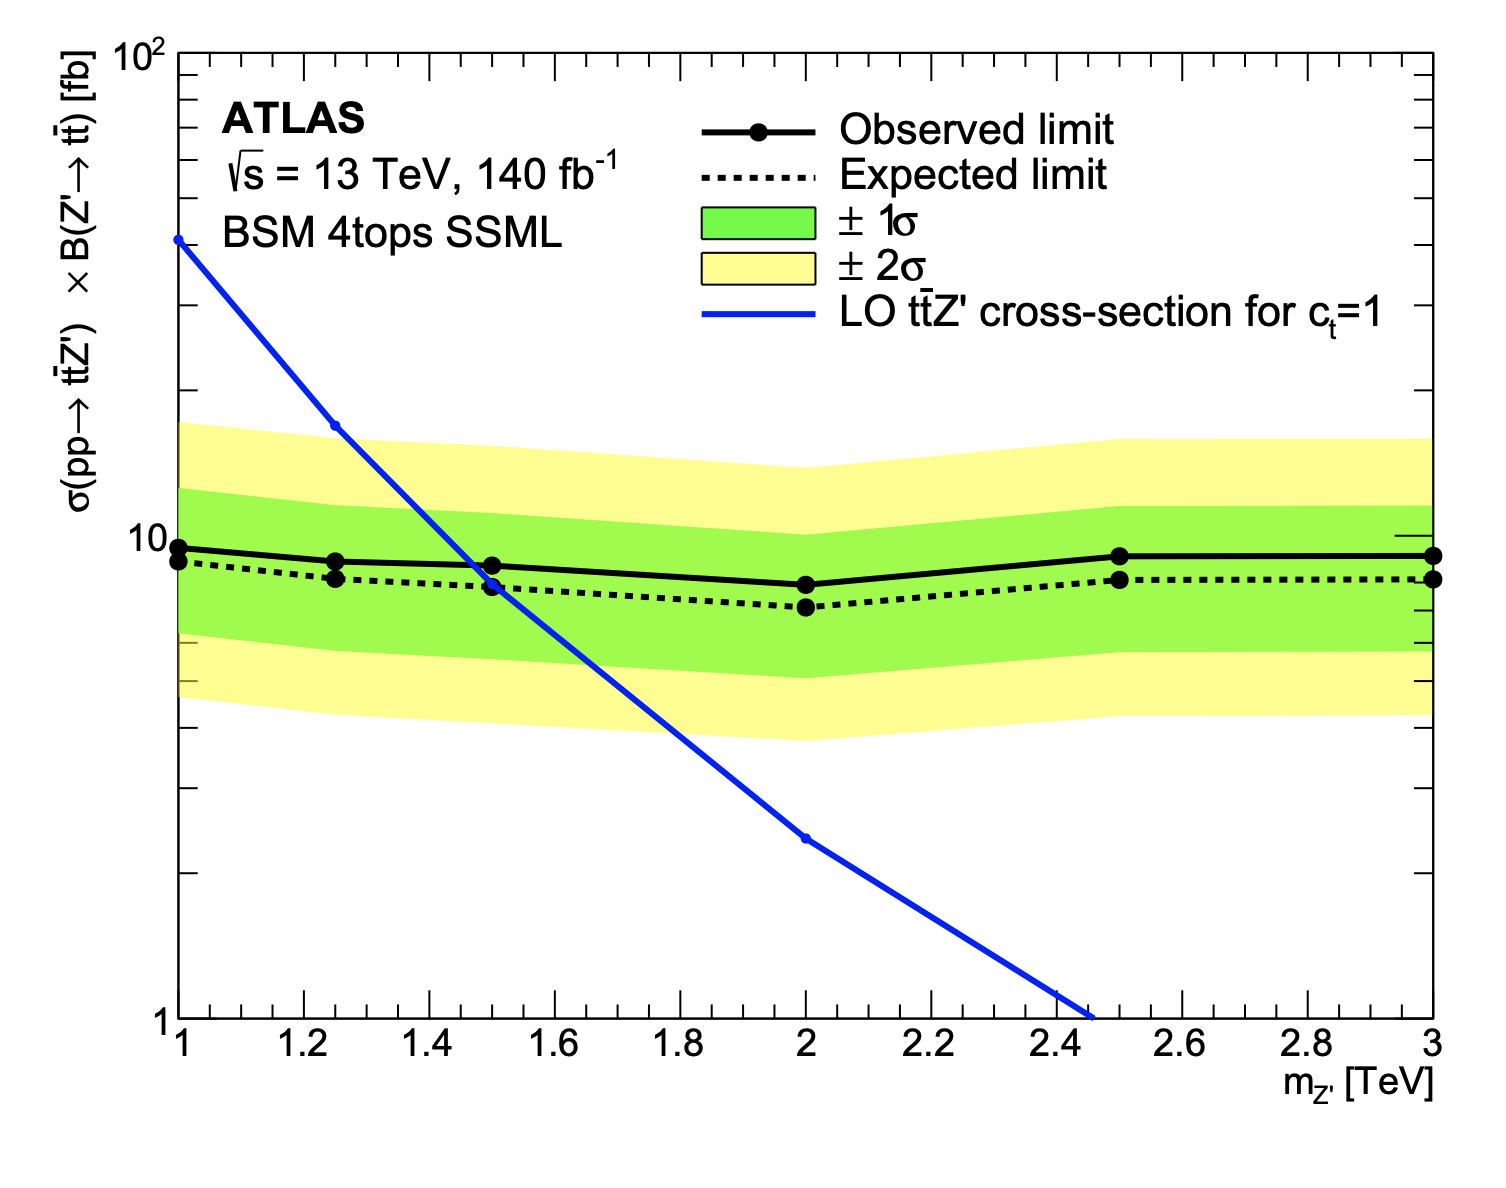
\includegraphics[width=0.8\linewidth]{fig/SRunblinded/ttZp_limits_fb.png}
\caption[Observed (solid line) and expected (dotted line) upper limits as a function of the $Z'$ mass at 95\% \acs{CL} on the cross-section of $pp\rightarrow\ttZp$ production times the $Z'\rightarrow\ttbar$ branching ratio. The region above the observed limit is excluded. The solid blue line represents the theoretical signal cross-section with $c_t=1$ at \acs{LO} in \acs{QCD}. The green and yellow bands represent the 68\% ($\pm\sigma$) and 95\% ($\pm 2\sigma$) confidence intervals respectively.]{\label{fig:results:ttZp_limits}Observed (solid line) and expected (dotted line) upper limits as a function of the $Z'$ mass at 95\% \acs{CL} on the cross-section of $pp\rightarrow\ttZp$ production times the $Z'\rightarrow\ttbar$ branching ratio. The region above the observed limit is excluded. The solid blue line represents the theoretical signal cross-section with $c_t=1$ at \acs{LO} in \acs{QCD} \citep{theory:ttZp_LHC}. The green and yellow bands represent the 68\% ($\pm 1\sigma$) and 95\% ($\pm 2\sigma$) confidence intervals for the expected upper limits.}
\end{figure}


\begin{table}[!htb]
\centering
\scriptsize
\setlength{\tabcolsep}{3pt} % Reduce column spacing
\renewcommand{\arraystretch}{1.2} % Adjust row spacing
\caption{\label{tab:results:NFs}Normalization factors for backgrounds with dedicated \acs{CR}s, obtained from a simultaneous fit in all \acs{CR}s and \acs{SR} under the background-only hypothesis. 
%Values shown are obtained from the fit using the \ttZp signal sample with $m_{Z'}=2$ TeV.
The nominal pre-fit value is 1 for all \acs{NF}s and 0 for the scaling factors $a_0$ and $a_1$. Uncertainties shown include both statistical and systematic uncertainties.}
\resizebox{\textwidth}{!}{%
\begin{tabular}{l|cccc|cccc}
\toprule
Parameter	& $\mathrm{NF}_{\text{HF }e}$	& $\mathrm{NF}_{\text{HF }\mu}$	& $\mathrm{NF}_{\text{Mat. Conv.}}$ & $\mathrm{NF}_{\text{Low }m_{\gamma^{*}}}$ & $a_0$ & $a_1$ & $\mathrm{NF}_{\ttWplus(4\mathrm{j})}$ & $\mathrm{NF}_{\ttWminus(4 \mathrm{j})}$ \\
\midrule
Fit value	& $0.68^{+0.23}_{-0.22}$ & $0.97^{+0.17}_{-0.16}$ & $0.97^{+0.31}_{-0.28}$ & $0.97^{+0.23}_{-0.20}$ & $0.39^{+0.11}_{-0.11}$ & $0.42^{+0.25}_{-0.24}$ & $1.21^{+0.18}_{-0.18}$ & $1.10^{+0.26}_{-0.26}$ \\
\bottomrule
\end{tabular}
}
\end{table}

% mZp2000
\begin{figure}[!htbp]
\centering
\subfloat[\CRttWm]{
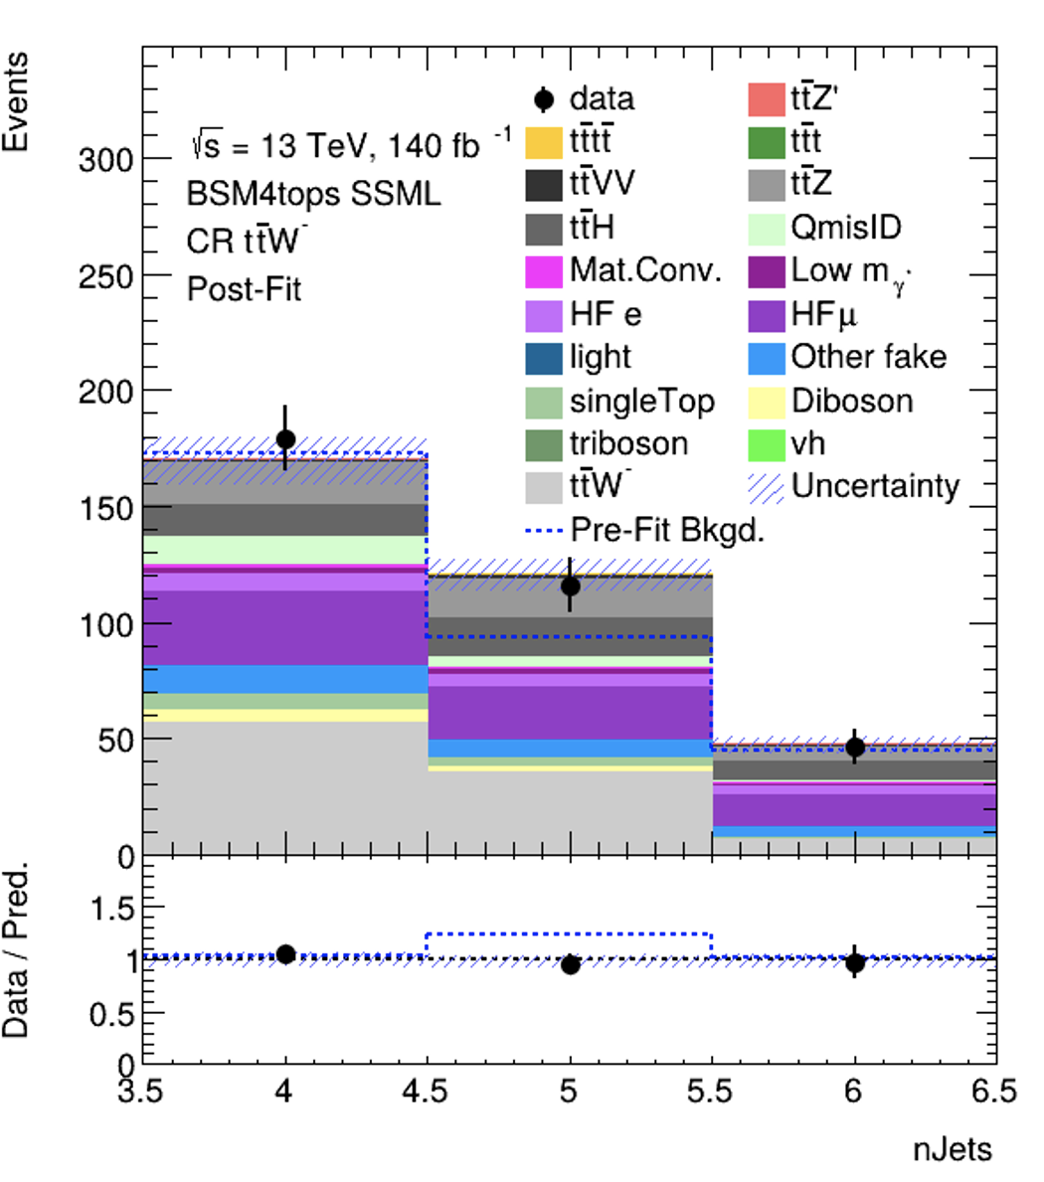
\includegraphics[width=0.32\linewidth]{fig/SRunblinded/CRttW2l_minus_nJets_postFit.png}}
\subfloat[\CRttWp]{
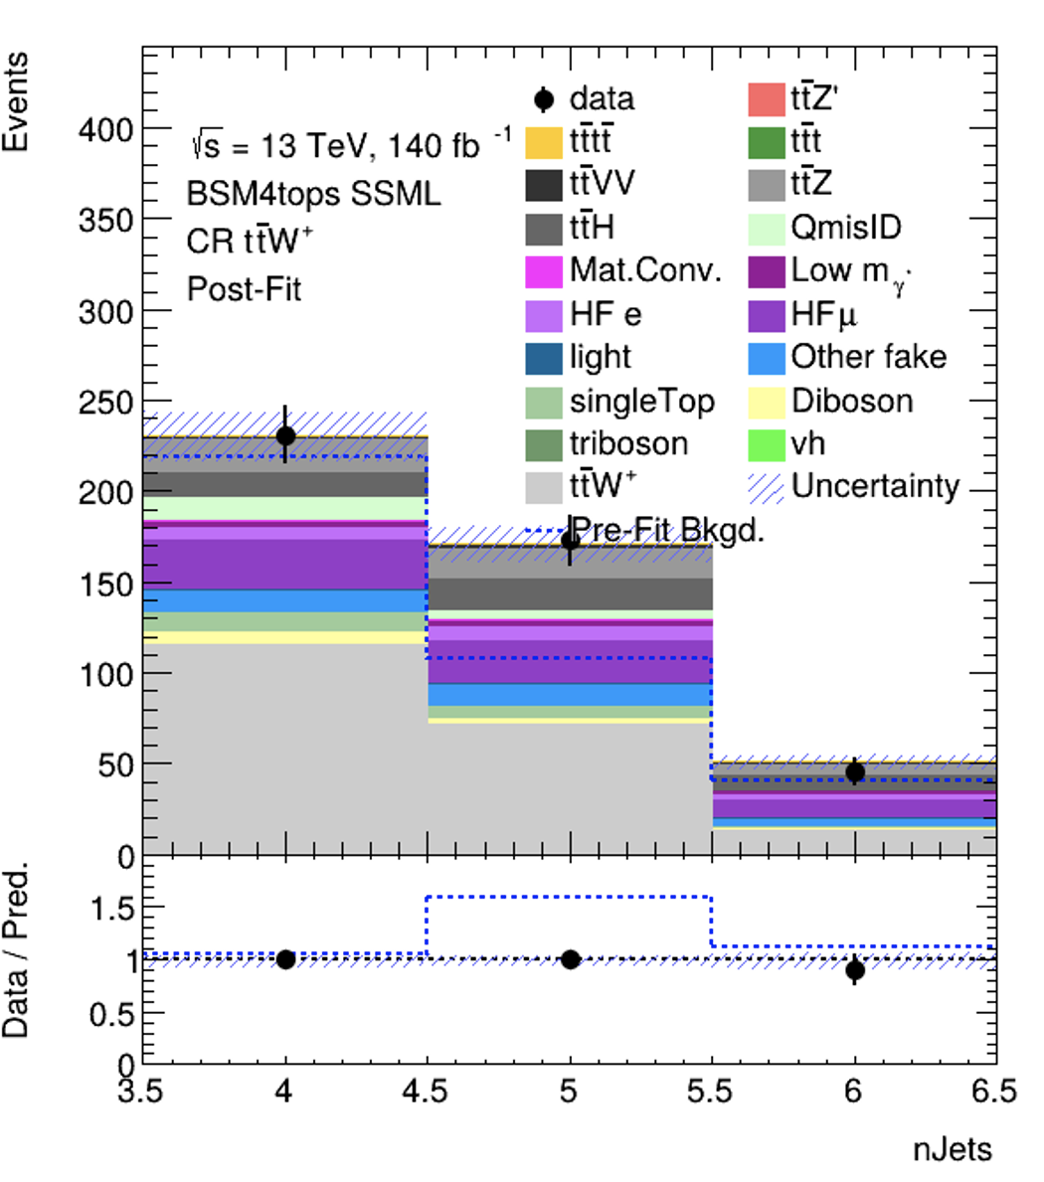
\includegraphics[width=0.32\linewidth]{fig/SRunblinded/CRttW2l_plus_nJets_postFit.png}}
\subfloat[\CRonebm]{
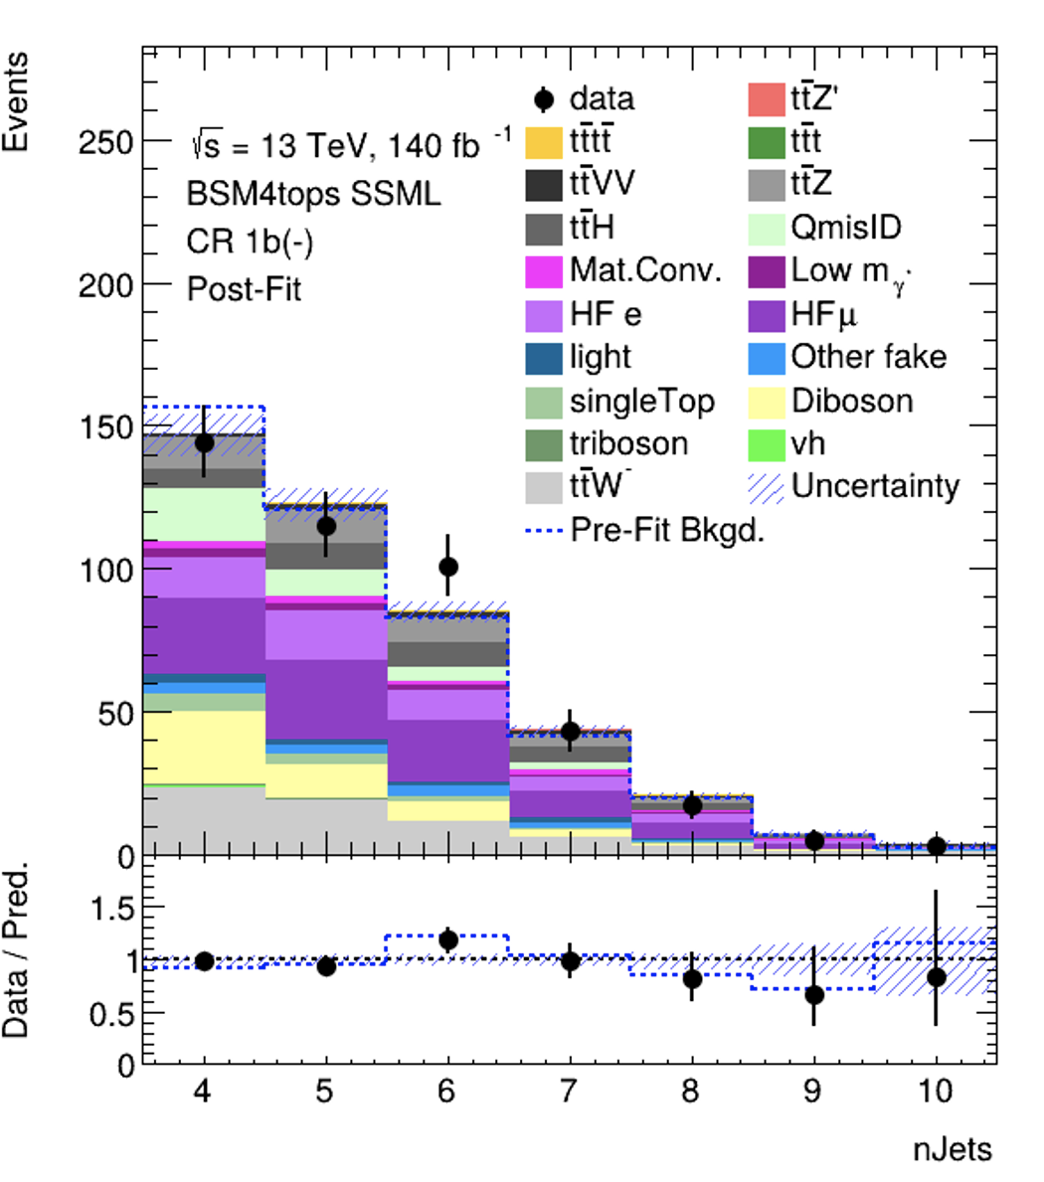
\includegraphics[width=0.32\linewidth]{fig/SRunblinded/CR1bminus_nJets_postFit.png}}

\subfloat[\CRonebp]{
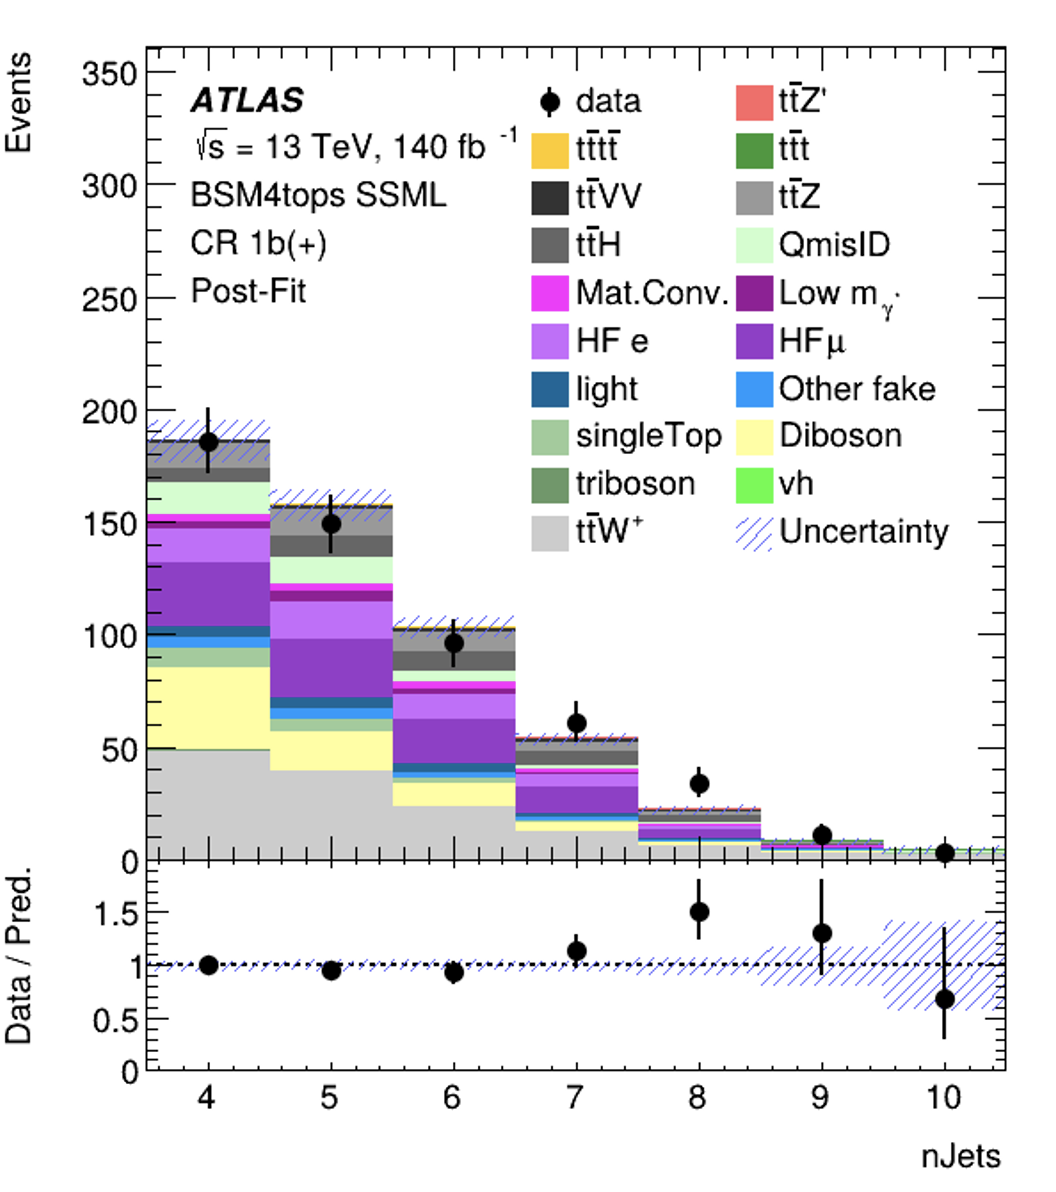
\includegraphics[width=0.32\linewidth]{fig/SRunblinded/CR1bplus_nJets_postFit.png}}
\subfloat[CR HF $e$]{
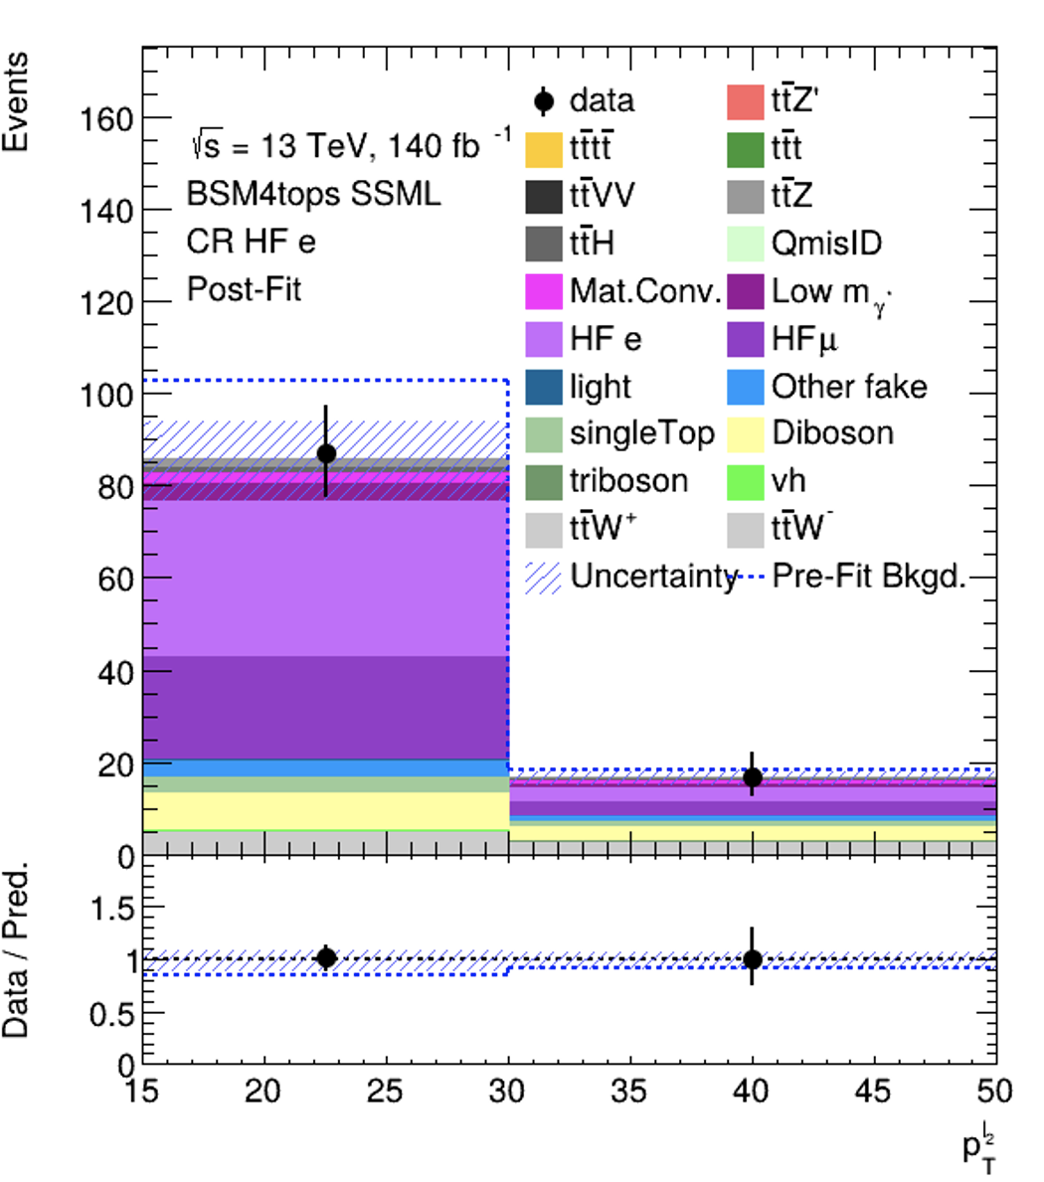
\includegraphics[width=0.32\linewidth]{fig/SRunblinded/CR1b3le_lep_2_pt_postFit.png}}
\subfloat[CR HF $\mu$]{
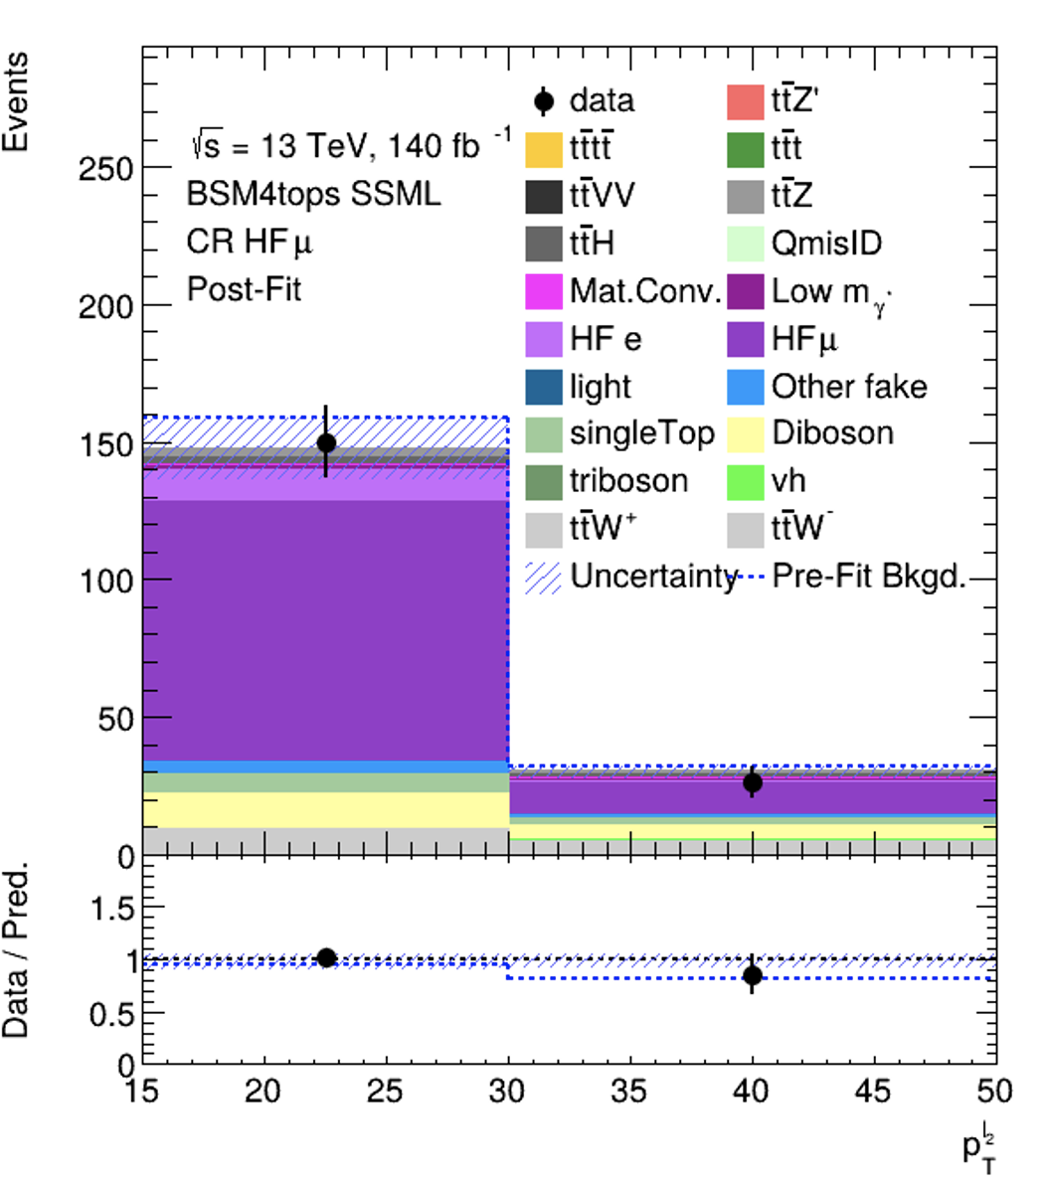
\includegraphics[width=0.32\linewidth]{fig/SRunblinded/CR1b3lm_lep_2_pt_postFit.png}}

\subfloat[CR Mat. Conv]{
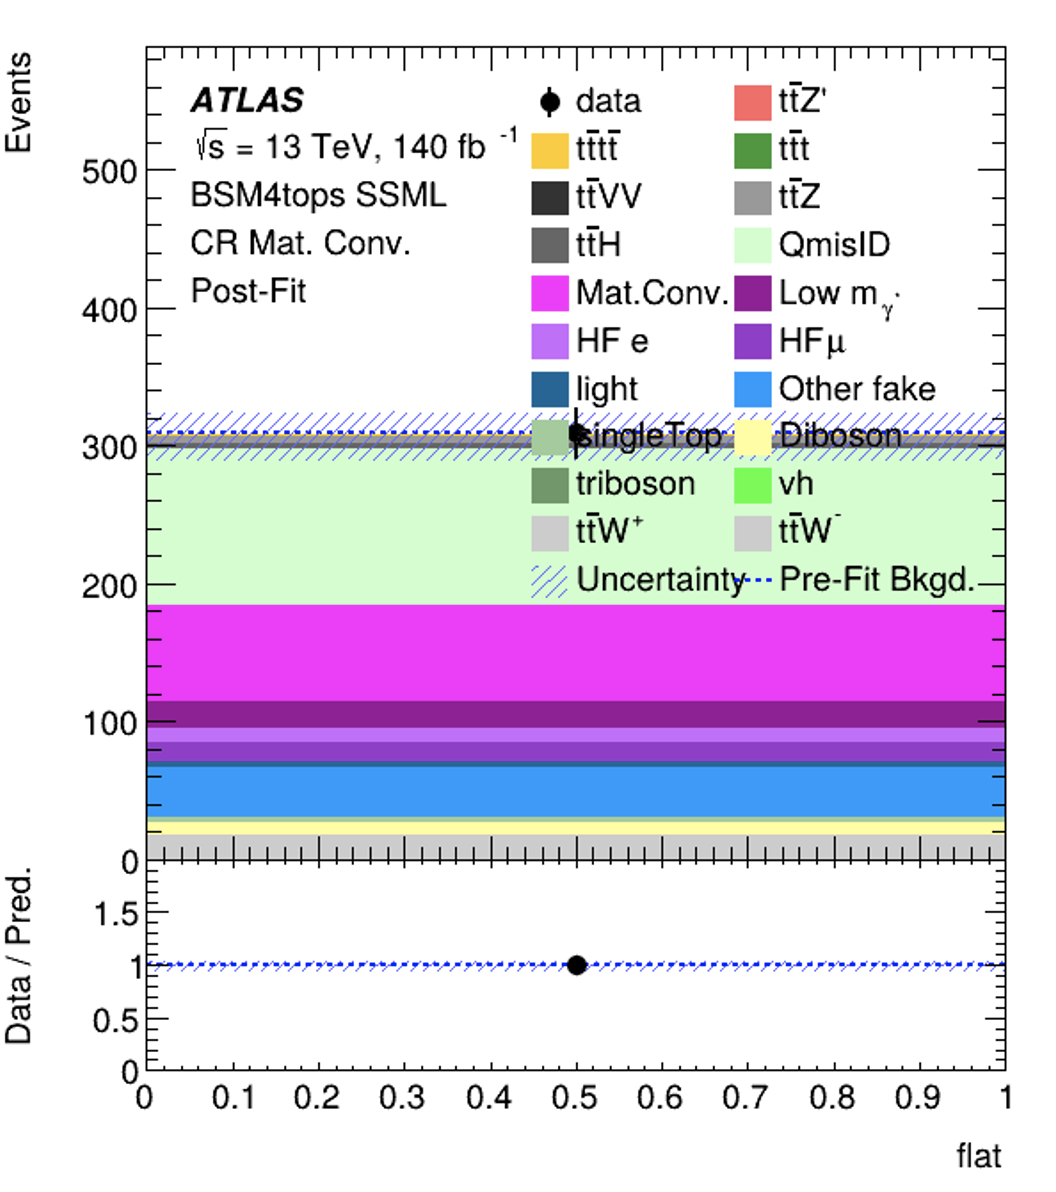
\includegraphics[width=0.32\linewidth]{fig/SRunblinded/CRttbarCO2l_CO_1_postFit.png}}
\subfloat[CR Low $m_{\gamma^*}$]{
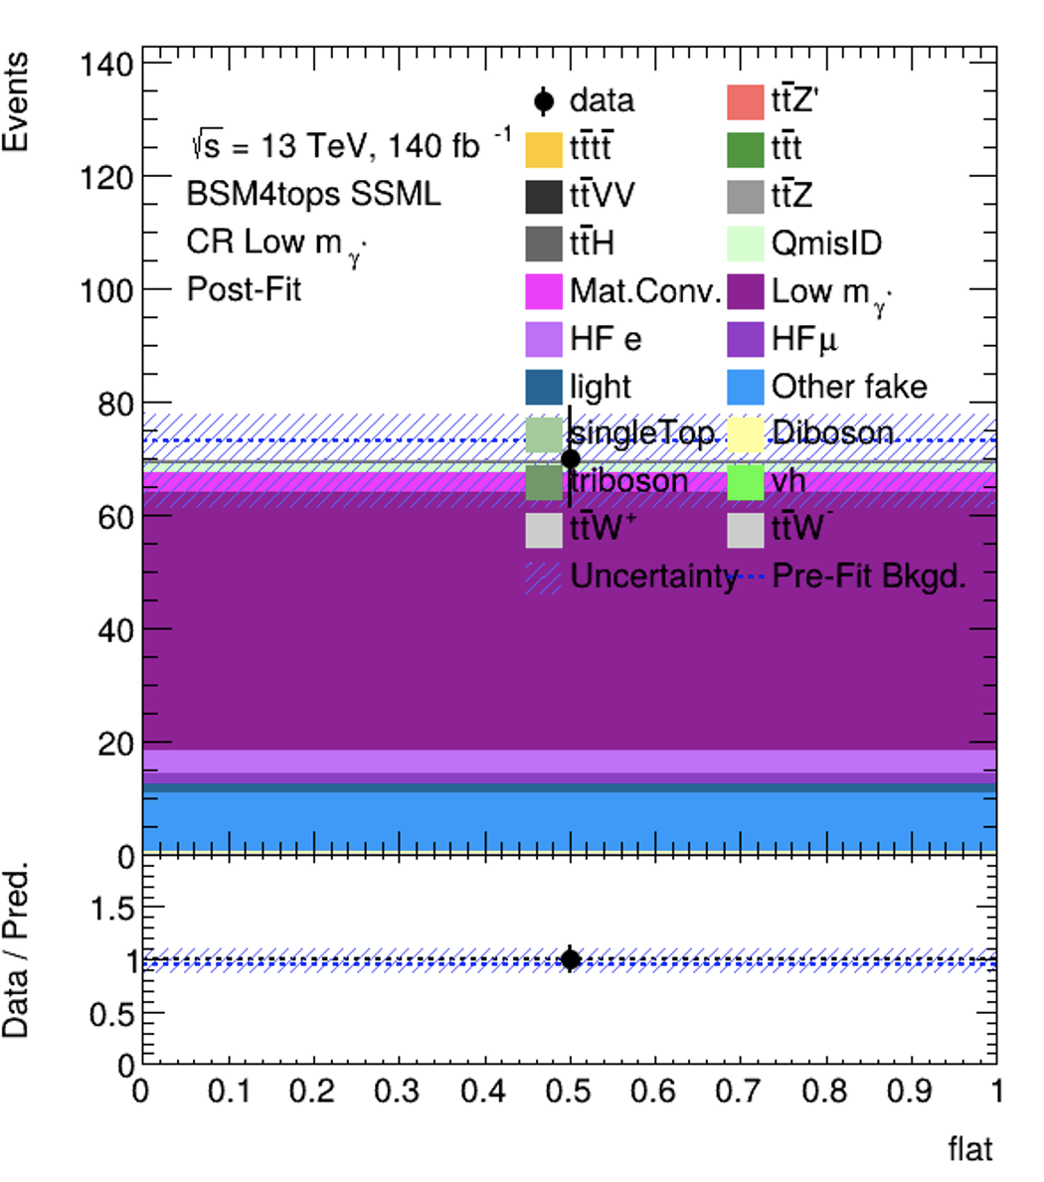
\includegraphics[width=0.32\linewidth]{fig/SRunblinded/CRttbarCO2l_gstr_1_postFit.png}}
\caption{\label{fig:results:bg_postfit}Comparison between data and post-fit prediction for the discriminant observable in each \acs{CR}. Distributions shown are obtained from the fit using the \ttZp signal sample with $m_{Z'}=2$ TeV. The lower panel shows the ratio between data and post-fit predictions. The shaded band represents the total uncertainty on the fit. The dashed line represents the pre-fit distribution.}
\end{figure}

\begin{table}[!htb]
  \centering
  \scriptsize
  \setlength{\tabcolsep}{8pt} % Reduce column spacing
  \renewcommand{\arraystretch}{1.2} % Adjust row spacing
  \caption{\label{tab:results:yield}Pre-fit and post-fit background yields in the inclusive \acs{SR}. The number of data events and pre-fit estimate signal yields are also shown. Background yields shown are obtained using the \ttZp signal sample with $m_{Z'}=2$ TeV. Pre-fit yields for \ttW background are set to 0 nominally prior to data-driven normalization. Total yield uncertainty differs from the quadrature sum of constituent uncertainties due to (anti-)correlation effects.}
  \resizebox{0.9\textwidth}{!}{%\
    \begin{tabular}{lcc}
      \toprule \midrule
      Process 					& Pre-fit 			& Post-fit	\\
      \midrule
      \multicolumn{3}{l}{\textbf{Background}} 	\\	
%      \midrule
      \tttt 					& 42.35 $\pm$ 5.45		& 46.91 $\pm$ 5.19 \\
      \ttWplus 					& -		& 103.93 $\pm$ 15.91 \\
      \ttWminus 				& -		& 55.27 $\pm$ 11.14 \\
      \ttZ 						& 78.02 $\pm$ 14.12		& 75.57 $\pm$ 11.13 \\
      \ttH 						& 81.00 $\pm$ 7.10		& 82.90 $\pm$ 7.30 \\
      \ttt 						& 3.33 $\pm$ 0.59		& 3.37 $\pm$ 0.60 \\
      Single-top ($tq$, $tZq$, $tWZ$, etc.)
      							& 13.38 $\pm$ 2.87		& 12.69 $\pm$ 2.86 \\
      \ttVV/\ttVH/\ttHH			& 17.07 $\pm$ 4.66		& 16.44 $\pm$ 4.64 \\
      Charge misidentification	& 40.31 $\pm$ 0.32		& 40.33 $\pm$ 0.32 \\
      $VV/VVV/VH$	 			& 10.01 $\pm$ 4.76		& 6.69 $\pm$ 2.75 \\
%      \midrule
      Mat. Conv. 				& 26.20 $\pm$ 0.91		& 25.76 $\pm$ 6.06 \\
      Low $m_{\gamma^{*}}$ 		& 26.14 $\pm$ 0.66		& 25.62 $\pm$ 4.23 \\
      HF $e$ 					& 21.99 $\pm$ 1.45		& 15.42 $\pm$ 3.70 \\
      HF $\mu$ 					& 31.33 $\pm$ 3.47		& 31.53 $\pm$ 5.06 \\
      Light-flavor decays 		& 13.47 $\pm$ 0.53		& 13.54 $\pm$ 0.53 \\
      Other fake \& non-prompt 	& 24.90 $\pm$ 2.26		& 26.00 $\pm$ 1.96 \\
      \midrule
      Total background		 	& -	& 576.53 $\pm$ 19.86 \\
      \midrule
      \multicolumn{3}{l}{\textbf{Signal $\ttZp \rightarrow \tttt$}} 	\\	
%      \midrule
      $m_{Z'}=1$ TeV 			& 52.83 $\pm$ 1.41		& - \\
      $m_{Z'}=1.25$ TeV 		& 52.94 $\pm$ 1.35		& - \\
      $m_{Z'}=1.5$ TeV 			& 53.07 $\pm$ 1.47		& - \\
      $m_{Z'}=2$ TeV 			& 52.49 $\pm$ 1.43		& - \\ %24.60 $\pm$ 7.14 \\
      $m_{Z'}=2.5$ TeV 			& 53.07 $\pm$ 1.47		& - \\
      $m_{Z'}=3$ TeV 			& 52.45 $\pm$ 1.50		& - \\
      \midrule
      \textbf{Data}				& \multicolumn{2}{c}{604} 		\\
      \midrule\bottomrule
    \end{tabular}
}
\end{table}

\begin{table}[!htb]
  \centering
  \scriptsize
%  \setlength{\tabcolsep}{3pt} % Reduce column spacing
  \renewcommand{\arraystretch}{1.2} % Adjust row spacing
  \caption{\label{tab:results:uncertainty}Post-fit impact of uncertainty sources on the signal strength $\mu$, grouped by categories. Values shown are obtained from the fit using the \ttZp signal sample with $m_{Z'}=2$ TeV. Impact on $\mu$ is evaluated for each uncertainty category by re-fitting with the corresponding set of \acs{NP}s fixed to their best-fit values. Total uncertainty differs from the quadrature sum of constituent uncertainties due to correlation between \acs{NP}s in the fit.} 
  \resizebox{0.9\textwidth}{!}{%\
    \begin{tabular}{lcc}
      \toprule \midrule
      Uncertainty source					& \multicolumn{2}{c}{$\Delta\mu$}	\\
      \midrule
      \multicolumn{3}{l}{\textbf{Signal modeling}} 	\\	%      \midrule
      \ttZp					 				& $+0.00$	& $-0.00$	\\
      \midrule
      \multicolumn{3}{l}{\textbf{Background modeling}} 	\\	%      \midrule
      \tttt 								& $+0.15$	& $-0.13$	\\
      \ttW	 								& $+0.04$	& $-0.03$	\\
      \ttZ									& $+0.02$	& $-0.02$	\\
      \ttH 									& $+0.02$	& $-0.02$	\\
      Non-prompt leptons					& $+0.00$	& $-0.00$	\\
      Other backgrounds						& $+0.02$	& $-0.02$	\\
      \midrule
      \multicolumn{3}{l}{\textbf{Instrumental}} 	\\	%      \midrule
      Luminosity							& $+0.00$	& $-0.00$	\\
      Jet uncertainties						& $+0.04$	& $-0.04$	\\
      Jet flavor tagging ($b$-jets)			& $+0.04$	& $-0.04$	\\
      Jet flavor tagging ($c$-jets)			& $+0.01$	& $-0.01$	\\
      Jet flavor tagging (light-jets)		& $+0.02$	& $-0.01$	\\
      \acs{MC} simulation sample size		& $+0.01$	& $-0.01$	\\
      Other experimental uncertainties		& $+0.01$	& $-0.01$	\\
      \midrule
      Total systematic uncertainty		 	& $+0.15$	& $-0.17$	\\
      \midrule
      \multicolumn{3}{l}{\textbf{Statistical}} 	\\	%      \midrule
%      Intrinsic statistical uncertainty		
%      										& $+0.25$	& $-0.23$	\\
      \ttW \acs{NF}s and scaling factors	
      										& $+0.01$	& $-0.01$	\\
      Non-prompt lepton \acs{NF}s (HF, Mat. Conv., Low $m_{\gamma^*}$)		
      										& $+0.00$	& $-0.00$	\\
      \midrule
      Total statistical uncertainty		 	
      										& $+0.25$	& $-0.23$	\\
      \midrule
      \textbf{Total uncertainty}			& $+0.29$	& $-0.29$	\\
      \midrule\bottomrule
    \end{tabular}
}
\end{table}




\end{document}